\begin{figure}[h!]
	\centering
	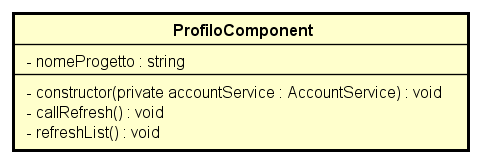
\includegraphics[scale=0.8]{res/sections/SpecificaFrontEnd/Components/Disegnetti/profilo.png}
	\caption{Diagramma della classe ProfiloComponent}
\end{figure}

\begin{itemize}
	\item \textbf{Descrizione:}\\
	È il componente che descrive la voce \textit{Profilo} del menu dell'editor.
	\item \textbf{Utilizzo:}\\
	Viene utilizzato dal MenuComponent per la gestione della voce profilo del menu.
	\item \textbf{Attributi:}
		\begin{itemize}
			\item \emph{-nomeProgetto: string}\\
			Contiene il nome del progetto corrente
		\end{itemize}
	\item \textbf{Metodi:}
		\begin{itemize}
			\item \emph{-constructor(private accountService: AccountService)}\\
    		Costruttore della classe\\
    		\textbf{Parametri:}
    		\begin{itemize}
    			\item \emph{accountService: AccountService}\\
    			Crea un istanziazione di AccountService
    		\end{itemize}
    		\item \emph{-callRefresh()}\\
    		Effettua la chiamata al metodo di aggiornamento della lista progetti\\
    		\item \emph{-refreshList()}\\
    		Aggiorna la lista progetti
		\end{itemize}
\end{itemize}